\section{FPGAs}

FPGA, ou Field Programmable Gate Arrays, são dispositivos eletrônicos que são baseados em matrizes de blocos lógicos configuráveis que são conectados via interconexões programáveis \cite{AmdFpga}. Eles podem ser programados e reprogramados para as funcionalidades desejadas.

Sua utilização é necessária em aplicações onde uma implementação em software utilizando um microcontrolador não é capaz de cumprir os requisitos de frequência de operação \cite{Sulaiman}.

O que cada bloco lógico possui internamente depende da fabricante e modelo do dispositivo, mas de forma geral possuem pelo menos Look-Up Tables (LUTs), que são implementações em hardware de tabelas verdade e elementos de memória, como Flip-Flops \cite{Sato}.

A Figura \ref{fig:FPGAStructure} ilustra a estrutura básica de um FPGA mostrando os blocos lógicos configuráveis, as conexões programáveis.

\begin{figure}[H]
    \centering
    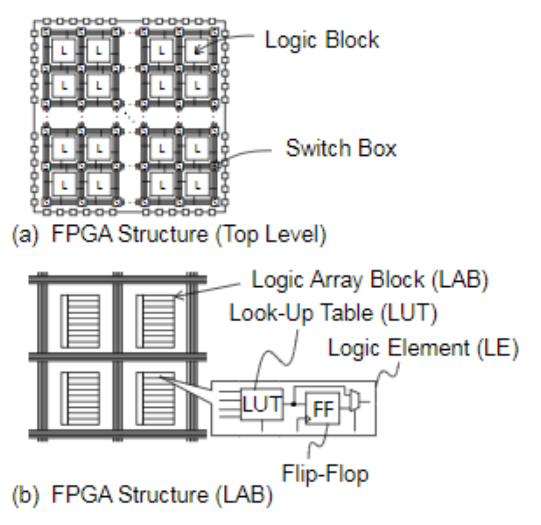
\includegraphics[scale=0.5]{figures/FPGAStructure.png}
    \caption{Estrutura de um FPGA. Fonte: \cite{Sato}}
    \label{fig:FPGAStructure}
\end{figure}

Os FPGAs são, de forma geral, programados utilizando linguagens de descrição de hardware (HDL), sendo VHDL e Verilog as mais utilizadas \cite{Ain}. Essas linguagens, diferentemente de linguagens de programação convencionais onde se escreve uma série de comandos que serão executados de maneira sequencial, descrevem um circuito elétrico que será sintetizado no dispositivo.

A linguagem Verilog permite descrever sistemas digitais desde o nível de portas lógicas ao nível de algoritmo. Também descreve um design do ponto de vista comportamental, de fluxo de dados, comportamental e de atrasos \cite{Bhasker}. Além disso, define sintaxe, semântica e estrutura para realizar simulações, facilitando os testes antes da prototipação e possui simbologia e estrutura parecida com a linguagem C, tornando-se mais familiar para quem for utilizá-la \cite{Wunnava}.
